
% Cal Poly Thesis
% 
% based on UC Thesis format
%
% modified by Mark Barry 2/07.
%

\documentclass[12pt]{ucthesis}

\usepackage{ifpdf} 
\newif\ifpdf
\ifx\pdfoutput\undefined
    \pdffalse % we are not running PDFLaTeX
\else
\pdfoutput=1 % we are running PDFLaTeX
\pdftrue \fi

\usepackage{url}
\usepackage{multicol}
\ifpdf

    \usepackage[pdftex]{graphicx}
    % Update title and author below...
    \usepackage[pdftex,plainpages=false,breaklinks=true,colorlinks=true,urlcolor=blue,citecolor=blue,%
                                       linkcolor=blue,bookmarks=true,bookmarksopen=true,%
                                       bookmarksopenlevel=3,pdfstartview=FitV,
                                       pdfauthor={Forrest Reiling},
                                       pdftitle={Extending Windowing Systems to Three Dimensions},
                                       pdfkeywords={thesis, masters, cal poly}
                                       ]{hyperref}
    %Options with pdfstartview are FitV, FitB and FitH
    \pdfcompresslevel=1

\else
    \usepackage{graphicx}
\fi

\usepackage{hyperref}
\hypersetup{
	linktoc=all,
    colorlinks,
    citecolor=black,
    filecolor=black,
    linkcolor=black,
    urlcolor=black
}



\usepackage{titlesec}
% \titleformat{\chapter}[display]% OLD
%     {\normalfont\huge\bfseries}{\chaptertitlename\ \thechapter}{20pt}{\Huge}% OLD
% \titlespacing*{\chapter}{0pt}{50pt}{40pt}% OLD
\titleformat{\chapter}[display]% NEW
    {\normalfont\centering}{\chaptertitlename\ \thechapter}{12pt}{}% NEW
\titlespacing*{\chapter}{0pt}{30pt}{20pt}% NEW

%\titleformat{\section}[block]{first}{label}{12pt}

\titleformat{\section}{}{\thesection}{1em}{}
\titleformat{\subsection}{}{\thesubsection}{1em}{}
\titleformat{\subsubsection}{}{\thesubsubsection}{1em}{}
\titleformat{\paragraph}{}{\theparagraph}{1em}{}

\usepackage[font={}]{caption}

%\renewcommand{\cftchapleader}{\cftdotfill{\cftdotsep}} % for chapters
%\renewcommand{\cftsecleader}{\cftdotfill{\cftdotsep}} 


\usepackage{amssymb}
\usepackage{amsmath}
\usepackage[letterpaper]{geometry}
\usepackage[overload]{textcase}
%\usepackage[toc,page]{appendix}

\usepackage{tabularx}
\usepackage{mdframed}
\usepackage{algpseudocode}
\usepackage{booktabs}
\usepackage{fixltx2e}


\usepackage{rotating}

\usepackage{enumitem}
\setlist{nolistsep}


\usepackage{float}
\floatstyle{boxed}
%\restylefloat{table}

\bibliographystyle{abbrv}

\setlength{\parindent}{0.25in} \setlength{\parskip}{6pt}

\geometry{verbose,nohead,tmargin=1.25in,bmargin=1in,lmargin=1.5in,rmargin=1.3in}

\setcounter{tocdepth}{4}
\setcounter{secnumdepth}{4}

% Different font in captions (single-spaced, bold) ------------
%\newcommand{\captionfonts}{\small\bf\ssp}
\newcommand{\captionfonts}{}

\makeatletter  % Allow the use of @ in command names
\long\def\@makecaption#1#2{%
  \vskip\abovecaptionskip
  \sbox\@tempboxa{{\captionfonts #1: #2}}%
  \ifdim \wd\@tempboxa >\hsize
    {\captionfonts #1: #2\par}
  \else
    \hbox to\hsize{\hfil\box\@tempboxa\hfil}%
  \fi
  \vskip\belowcaptionskip}
\makeatother   % Cancel the effect of \makeatletter
% ---------------------------------------



\begin{document}

% Declarations for Front Matter

% Update fields below!
\title{Optimizing Lempel-Ziv Factorization for the GPU Architecture}
\author{Bryan Ching}
\degreemonth{June} \degreeyear{2014} \degree{Master of Science}
\defensemonth{June} \defenseyear{2014}
\numberofmembers{3} \chair{Assistant Professor Chris Lupo, Ph.D.,\newline Department of Computer Science} \othermemberA{Associate Professor John Seng, Ph.D.,\newline Department of Computer Science} \othermemberB{Assistant Professor Zachary N J Peterson, Ph.D.,\newline Department of Computer Science} \field{Computer Science} \campus{San Luis Obispo}
\copyrightyears{seven}



\maketitle

\begin{frontmatter}

% Custom made for Cal Poly (by Mark Barry, modified by Andrew Tsui).
\copyrightpage

% Custom made for Cal Poly (by Andrew Tsui).
\committeemembershippage

\begin{abstract}
Lossless data compression is used to reduce storage requirements, allowing for the relief of I/O channels and better utilization of bandwidth.
The Lempel-Ziv lossless compression algorithms form the basis for many of the most commonly used compression schemes.
General purpose computing on graphic processing units (GPGPUs) allows us to take advantage of the massively parallel nature of GPUs for computations other that their original purpose of rendering graphics. 
Our work targets the use of GPUs for general lossless data compression.
Specifically, we developed and ported an algorithm that constructs the Lempel-Ziv factorization directly on the GPU.
Our implementation bypasses the sequential nature of the LZ factorization and attempts to compute the factorization in parallel.
By breaking down the LZ factorization into what we call the PLZ, we are able to outperform the fastest serial CPU implementations by up to 24x and perform comparatively to a parallel multicore CPU implementation.
To achieve these speeds, our implementation outputted LZ factorizations that were on average only 0.01 percent greater than the optimal solution that what could be computed sequentially.

We are also able to reevaluate the fastest GPU suffix array construction algorithm, which is needed to compute the LZ factorization.
We are able to find speedups of up to 5x over the fastest CPU implementations.

\end{abstract}


\begin{acknowledgements}

Thanks to:

\begin{itemize}
\item My advisor Chris Lupo, for all of his guidance and patience and for introducing me to the GPGPU.
\item My parents, my family, and everyone who has supported me to where I am today.
\end{itemize}

\end{acknowledgements}

\tableofcontents

\listoftables

\listoffigures

\end{frontmatter}

\pagestyle{plain}

\renewcommand{\baselinestretch}{1.66}


% ------------- Main chapters here --------------------
\chapter{Introduction}
The space we exist in is three dimensional, and this pervades every aspect of our interaction with reality. Everything we touch, see, and hear behaves according to the rules of this three dimensional space and this has made humans exceptionally proficient at reasoning about it, navigating through it, and modelling the behaviour of things within it. Yet when we interact with our computers, an increasingly important part of our everyday lives, most of us do so exclusively through two dimensional user interfaces. 
 
\section{Two Dimensional User Interfaces}

The two dimensional space in which we interact with computers has come to define these interactions in the same way that the three dimensional space in which we exist defines our interaction with reality. We use our fingers or a mouse press 2D buttons and open 2D menus, driving change in the application’s 2D interfaces which the windowing system composites into a 2D image to be sent to a 2D display. While this is natural for some intrinsically 2D concepts, like documents and images, other concepts which have no intrinsic spatial embedding, like file systems and networks, are also embedded in 2D when they are presented to the user in order to allow users to reason about them spatially. Even in applications which are intrinsically 3D, like physical simulation and modelling tools, the 3D application space is disjoint from the space in which the user exists (by necessity, since the application has no knowledge of the 3D relationship between the display and the user) and interaction between the 3D application space and the 3D user is traditionally done with 2D input events and 2D images.  
	
The flat nature of contemporary graphical user interfaces has come to define not just the way we interact with applications, but has also become an important factor in the physical design of the computers that run these applications. This is particularly apparent in the mobile computer space, where cost, weight, display power, and mobility concerns push devices toward ever smaller physical profiles, while usability concerns drive the devices toward larger interface surfaces, leading the profile of mobile computers to become flattened against their displays, with the devices acting as a physical embedding of the 2D computer interface within the 3D space in which the computer exists. This forces users to make a tradeoff between the physical profile of their device and the usable size of their interface; larger displays drive up mass both directly and through the need for a larger battery to meet increased power demands, but a smaller displays limit the usable size of the human-computer interface which limits the usability of the device [citation needed]. In desktop computers the same tradeoff must be made, because even absent power and weight concerns the size of the interface is still constrained by the cost of the displays and the physical space needed to mount them in view of the user.

Two dimensional user interfaces are certainly not all bad. There is a natural analog between interacting with documents, images, and folders on a desk and interacting with their digital counterparts on a 2D display (which forms the underpinnings of the familiar desktop metaphor). 2D interfaces also map well onto commercially available display hardware as a result of the two co-evolving for several decades, which keeps the hardware cost of 2D interfaces relatively low. 2D interfaces are mature and well studied, and there is a rich software ecosystem surrounding them which includes sophisticated, full featured user interface toolkits and advanced windowing systems, as well as a broad set of end user applications that provide 2D graphical frontends for almost every task a user need perform on a computer. Users are also familiar with the operation of 2D interfaces, which greatly reduces the time needed for users to learn new applications and improves their productivity with existing applications. 

There are certain applications, like document and photo editing and command line interaction, which fit well with 2D interfaces, and in these applications moving away from 2D interactions would likely be detrimental. However, many applications are intrinsically 3D, or are not intrinsically spatial at all and are embedded in a 2D space because it is simple and well supported, and a transition to 3D interaction has the potential to greatly improve  the usability of such applications \cite{bowman_theory_practice}.

\section{Three Dimensional User Interfaces}

The hardware, software, and theory surrounding high quality 3D human-computer interaction has been the subject of academic research for many decades, and the improved spatial reasoning this provides has been demonstrated to improve usability in a  number of applications  \cite{bowman_theory_practice}. 3D user interfaces are a broad group of interaction paradigms, including everything from desktop 3D modeling with a mouse and keyboard to fully immersive virtual reality.  This thesis focuses on ‘immersive’ 3D interfaces, which is used here to refer to 3D interfaces in which the user perceives the 3D interface elements to be in the same 3D space as their body, and has some way of manipulating these interface elements in 3D with corresponding 3D motion by some part of their body.  The hardware needed to support these types of interfaces has traditionally been very expensive, but recent technological improvements in a number of fields have brought many of the core hardware technologies onto the consumer market, bringing both high quality 3D input devices and immersive 3D displays into the reach of everyday computer users.

\subsection{Three Dimensional Input Devices}

Early 3D input devices to come into the consumer 3D interaction market were largely marketed as video game accessories, though their availability has led to their use in a wide variety of other application. These devices can be broadly categorized into two groups: devices which resolve the position and/or orientation of an element held or worn by the user, and range-imaging cameras, which produce a 3D image of a passive scene which contains no sensing elements itself.

The first category had its first commercial success in consumer markets in 2006, when Nintendo introduced the Wii Remote, or ‘Wiimote’, as the primary controller for its new Wii entertainment system. This controller, unlike traditional game console controllers, was able to sense its position, orientation, and acceleration along 3 axes. The Wiimote provided limited 3D control within Wii games, and was soon adopted by developers for a wider variety of tasks, including controlling the visualization of volumetric medical data \cite{wiimote-medical} and enabling head tracking 3D on traditional displays \cite{hacking-the-wiimote}. Several devices which provided similar input using a variety of different tracking technologies soon came to market, including Sony’s “Playstation Move” in 2009, and the “Razer Hydra” in 2011 (Produced by Sixense Entertainment in partnership with Razer USA). Until the time of this writing all commercially available, consumer grade, 3D tracking solutions have been handheld controllers gripped by the user, but two new multi-sensor, wearable, full-body tracking solutions (Sixense’s new magnetic tracking system, STEM, and PrioVR’s inertial tracking system) are due to become commercially available within the next year in response to an emerging consumer virtual reality market.
 
Range imaging cameras can be based on a variety of technologies, many of which have been commercially available for many years but have been too expensive to be accessible to a wide body of consumers. In 2009, following advances in real-time structured-light 3D scanning by Primesense Ltd, Microsoft released a range imaging camera based on a Primesense sensor to the public, under the name ‘Kinect’, as an accessory for their Xbox 360 game console. Designed to perform full body tracking in 3D on multiple users, the Kinect enabled a variety of new interaction techniques in Xbox games. Like the Wiimote, the Kinect was quickly adopted by third party developers and applied to numerous non-gaming domains, including robotics applications like Simultaneous Location and Mapping \cite{iser-rgbd-slam}, and a variety of medical applications \cite{kinect-medical}. Although the Kinect has received a great deal of attention, being the first consumer grade sensor capable of producing high quality images in real time, many other sensors have since come to market which offer comparable or better performance in a variety of applications and operating conditions. Primesense Ltd., the company that developed the technology underpinning the first generation Kinect, also developed sensors based on the same technology that were released both directly by Primesense under the name Carmine, and through Asus as the Xtion  and Xtion Live, which all offer very similar performance to the first generation Kinect \cite{depth-sensor-comparison}. Very recently, several consumer-grade range imaging cameras have become commercially available which rely on ‘time-of-flight’ technology, which has several advantages over structured lighting including lower software overhead, faster response time, and better bright light performance \cite{ti-tof}. This includes Microsoft’s next generation Kinect, released with the Xbox One in 2013, and the DS310 and DS325 from Belgium based SoftKinetic. The SoftKinetic DS325, also sold re-branded as the Creative Senz3D, is designed for close interaction and finger tracking rather than full body tracking \cite{softkinetc-products}, and competes in the consumer market with the Leap Motion, a desktop stereo camera designed specifically for hand, finger and stylus tracking in the space immediately above the keyboard. Several other companies, notably Texas Instruments and pmdVision, provide Time of Flight solutions, but to the author’s knowledge they do not sell consumer time of flight products as of the time of this writing. 
This is by no means an exhaustive list of 3D input devices; it is meant only to demonstrate the growing diversity of 3D input devices reaching the consumer market, and that this is a relatively recent development. At the surface level, these devices appear to produce a wide variety of input, but when constrained to human-computer interaction applications it becomes apparent that simple input models can capture the useful input produced by all of these devices. Essentially this is because the only mechanism humans have to produce 3D input is the movement of their body through the 3D space or the use of this movement to move an object through 3D space, which can be captured, respectively, by the notions of skeletal tracking and 3D pointing devices [cite Jester].

\subsection{Immersive Three Dimensional Displays}
	
	The term "3D display" has come to refer to a very broad category of devices, so the term "immersive 3D display" is used here to refer to graphical displays which support both stereo parallax (rendering the scene from a separate viewpoint for each eye) and head-tracking motion parallax (adjusting the position and orientation of these viewpoints based on the 3D relationship between the user and the display), as both are required to create a convincing 3D experience for the user (This is discussed in more detail in the background section). This excludes commercial 3D televisions and 3D movie theaters because they do not provide head tracking, and excludes haptic and audio ‘displays’ because they are not graphical. There have been many systems which meet these requirements in research and industrial applications, including Responsive Workbenches [citation], Hemispherical Displays [citation], CAVE Automated Virtual Environments (CAVEs) [citation], and Head Mounted Displays (HMDs) [citation], and some of these technologies, particularly CAVEs and HMD’s, have received significant research and developments, allowing the technology to mature significantly. 
Most of these technologies have remained outside of consumer reach, largely due to the large size and high cost of such systems, with the exception of HMDs, whose simplicity and compact design has led them to enjoy intermittent commercial availability for many years. A comprehensive discussion of commercially available HMDs is outside the scope of this paper, but it is worth noting that the recent release of OculusVR’s ‘Oculus Rift’ development kit to consumer markets has sparked a resurgence in interest in virtual reality for video games and other entertainment applications, leading to the announcement of several new consumer HMDs, including a consumer version of the Oculus Rift [citation], Sony’s ‘Project Morpheus’ [citation], and True Player Gear’s ‘Totem’ [citation]. 

Priced at only a few hundred dollars, these HMDs put high resolution, wide field-of-view, immersive 3D display technology in the hands of everyday computer users, and the continuing advances of consumer graphics processing hardware gives them the ability to drive convincing 3D scenes onto these displays with commodity hardware. Furthermore, like 3D input devices, the similarity in function between these devices means their behavior can be captured abstractly by relatively simple input and output models. 

\chapter{Background}

\section{GPU Architecture}

\section{Compression}

\subsection{Lempel Ziv Factorization}
The LZ factorization of a string S[n] decomposes S into factors S = w1w2. . . wk where k<=n, where each factor wi is either the longest factor that appears left of wi in S or is a new character. For example, the LZ factorization of string abbaabbbaaabab has the factorization a.b.b.a.abb.baa.ab.ab. This can be encoded simply with a position of previous occurence and the length of the match or a character, if the length is 0. Practical compression schemes might be encoded in triplets with the position, length, and the first letter of mismatch. Various algorithms have been compared experimentally in \cite{ }. In general, LZ factorization algorithms all make use of a few common data structures and stages, the suffix array, the LCP array, and the LPF array. 

\subsubsection{Suffix Array}

The suffix array is a common data structure in string matching algorithms. The suffix array SA of S is a lexicicographically ordered array of integers of size n where each integer represents a suffix of S, so that suf[SA[0]] < suf[SA[1]] < . . .  suf[SA[n-1]].

Suffix tree applications.

Suffix tree talk.

Various algorithms exist for the construction of suffix arrays. The skew algorithm of Kark \cite{ } uses a divide and conquer approach to construct a partial suffix array to infer the rest of the positions. Running in linear time, the skew algorithm has also been studied in parallel. The fastest known construction of suffix arrays on the GPU by Meo and Deeeley utilizes the skew algorithm. Our work is also a reimplementation and benchmark of that algorithm inspired by most of their ideas.

\subsubsection{LCP and LPF Array}

The LCP, longest common prefix, array is an auxiliary structure to the suffix array that provides the longest common prefix between successive suffixes in SA. Formally, position i in the LCP array, LCP[i] = lcp(suf[SA[i-1]],suf[SA[i]]).

The LPF, longest previous factor, array holds the lengths of the longest factors at any position i. In other words, LPF[i] holds the maximum lcp of suf[sa[i]] and all suffixes less than i.

\subsubsection{LZ Factorization Calculation}

Previous works have computed the LPF array from the LCP array using ranged minimum queries. More recent works do a lazy computation.

The lz factorization can be computed by following the lpf array.

% http://delivery.acm.org.ezproxy.lib.calpoly.edu/10.1145/2380000/2379781/a5-al-hafeedh.pdf?ip=129.65.23.208&id=2379781&acc=ACTIVE%20SERVICE&key=F26C2ADAC1542D74%2E2870C5A035FC0FDB%2E4D4702B0C3E38B35%2E4D4702B0C3E38B35&CFID=343020533&CFTOKEN=37720775&__acm__=1400733002_66a60490d28a219a079b67ccd7c8315e

\chapter{Implementation}
\label{sec:implementation}
This section describes the implementation of the design discussed in Section~\ref{sec:design} built on top of the Wayland display server protocol. This implementation, called `Motorcar`, is free and open source and available on GitHub \cite{motorcar-github}. It is intended both to demonstrate concretely that such a design is practical to implement, as well as to serve as a functional 3D windowing system and provide a modular core of that can form the basis of further research into the concept of 3D windowing systems.

\section{Wayland Protocol Extensions}

The design outlined in Section~\ref{sec:design} requires several pieces of functionality not provided by the core Wayland protocol (like synchronization of the view and projection matrices between the compositor and the clients) and functionality that is not supported by the subsystems on which Wayland in built (like the ability for the compositor to access client depth buffers)
\chapter{Results}
\label{chap:results}

\section{Experimental Setup}
\subsection{Test Machine}
All measurements were gathered from a single machine with an NVIDIA Tesla K40c and NVIDIA GTX TITAN Black.
The Tesla K40c and GTX TITAN Black are two of NVIDIA's higher end solutions.
The GTX TITAN Black, which we'll now refer to as Black, has a 0.98 GHz GPU clock rate, 3.5 GHz memory clock rate, and 6 GB of memory.
The Tesla K40c, now K40c, has a 0.88 GHz GPU clock rate, 3.0 GHz memory clock rate, and 12 GB of memory.
The Black is faster than the K40c, but has significantly less memory.
Both the CUDA runtime and driver version were 6.0.
The binary was compiled using -O3 optimization and compute capability 2.0.
Timings were recorded using the CUDA events API.

\subsection{Data}

Data for our evaluation was gathered from various publicly available datasets, often used in benchmarking lossless compression algorithms.

\section{Suffix Array}

\begin{figure}[ht!]
\centering
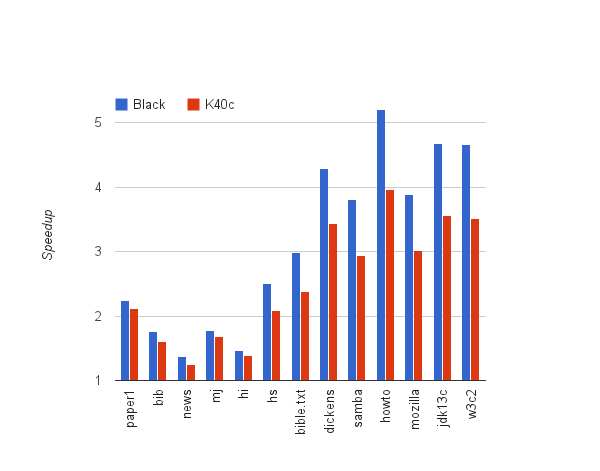
\includegraphics[width=1.0\textwidth]{images/saresult.png}
\caption{Speedup of GPU implementation to fastest CPU implementation}
\label{fig:saresult}
\end{figure}

\begin{table}[h]
\begin{tabular}{@{}lllllll@{}}
\toprule
size(MB) & filename  & Black  & K40c   & CPU   & Black Speedup & Black ms/input \\ \midrule
0.05     & paper1    & 15.2   & 16     & 34    & 2.2           & 0.286          \\
0.11     & bib       & 19.3   & 21.2   & 34    & 1.8           & 0.173          \\
0.36     & news      & 33.6   & 36.8   & 46    & 1.4           & 0.089          \\
0.43     & mj        & 29.2   & 30.9   & 52    & 1.8           & 0.065          \\
0.49     & hi        & 34.2   & 36.1   & 50    & 1.5           & 0.067          \\
3.14     & hs        & 108.5  & 130.6  & 272   & 2.5           & 0.033          \\
3.86     & bible.txt & 112.9  & 141.5  & 338   & 3.0           & 0.028          \\
9.72     & dickens   & 282.8  & 353.5  & 1212  & 4.3           & 0.028          \\
20.61    & samba     & 536.9  & 693    & 2042  & 3.8           & 0.025          \\
37.60    & howto     & 1021.1 & 1339.7 & 5320  & 5.2           & 0.026          \\
48.85    & mozilla   & 1278.2 & 1642.6 & 4958  & 3.9           & 0.025          \\
66.50    & jdk13c    & 1928.2 & 2525.4 & 9010  & 4.7           & 0.028          \\
99.37    & w3c2      & 2896   & 3840.8 & 13486 & 4.7           & 0.028          \\ \bottomrule
\end{tabular}
\caption{Runtimes(ms), speedups, and ms/input of datasets for evaluation of suffix array construction}
\label{tab:sadata}
\end{table}

The evaluation of the suffix array is actually an evaluation of a reimplementation of the fastest known GPU suffix array construction algorithm (SACA) by Deo and Keely\cite{Deo}.
The benefits and applications of the suffix array has already been detailed in chapter . . .
Deo and Keely's evaluation was done on an AMD Radeon GPU using OpenCL.
Our results on a NVIDIA GPU using CUDA and CUB primitives with ModernGPU's merge path method to mergesort are not expected to be significantly different.
We will be comparing out results to a set of SACA benchmarks found on the wiki of libdivsufsort, one of if not the fastest CPU SACA implementation \cite{ }.
That benchmark compares the fastest CPU SACA implementations on a variety of test files.
We will compare our GPU implementaion against the fastest CPU time for each file.
Files were picked to match closely with Deo and Keely's evaluation.
GPU times include parsing the file, transfering the data both ways, and the construction of the suffix array.

Figure~\ref{fig:saresult} and Table~\ref{tab:sadata} presents the results comparing the CPU implementations to our GPU implementation.
The first thing to note is that the CPU SACA benchmarks are significantly faster than those used by Deo and Keely.
Our GPU implementation did not see the speedup of 35x that theirs did, but we still found around a 4-5x speedup for most files for Black.
We did not have their implementation or their raw result data to compare against.
Loosely comparing with the charts in their paper though, we find that our GPU implementation is at least on par if not faster.

Another interesting metric is the runtime in microseconds per input symbol seen in \cite{ }.
We found that after a certain point, our Blakc was achieving rates of around 0.02 to 0.03 ms per input symbol.

Like many other GPU algorithms, we found that smaller files did not see the greater speedups that larger files did.
The likely cause is that smaller files cannot fully saturate the GPU, and the cost of initialization and data transfer could not be hidden by increased computations.
This indicates that the GPU is not the all around solution for faster suffix arrays and the size of the input needs to be considered.

\begin{figure}[ht!]
\centering
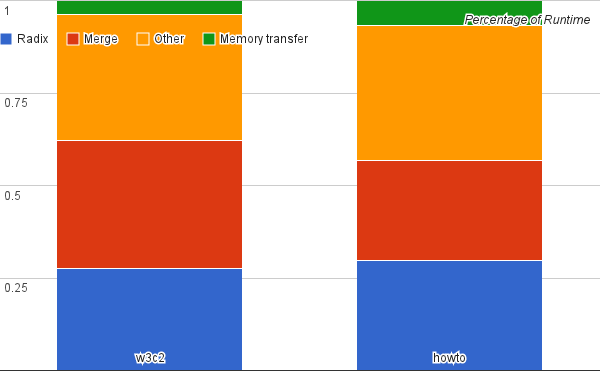
\includegraphics[width=1.0\textwidth]{images/saprofile.png}
\caption{Profile of Suffix Array construction on the GPU}
\label{fig:saprofile}
\end{figure}

Figure~\ref{fig:saprofile} shows a profile of the SACA of the GPU implementation.
Kernels other than those involved in the merging or sorting take the greatest percentage of time in both examples.
These kernels have the most room for improvement, since they are less likely to deal with primitives and more likely deal with the setup and movement of data.
The CUDA grid and block sizes could have a greater factor in the speeds and further optimization are more likely to see gains here.

aug 24 2008

\section{ANSV}

\begin{figure}[ht!]
\centering
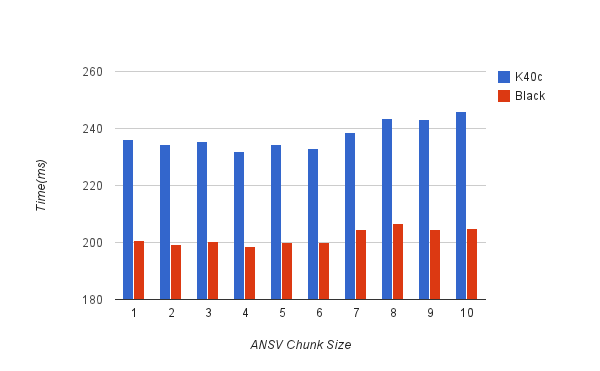
\includegraphics[width=1.0\textwidth]{images/ansvsize.png}
\caption{The effect of chunk size on ANSV runtime on the GPU}
\label{fig:ansvresult}
\end{figure}

As discussed in chapter X, the ANSV algorithm divides the suffix array into chunks for each thread.
These threads will then individually solve the ANSV problem on their chunk and solve any outliers using a preconstructed binary tree.

Figure~\ref{fig:ansvresult} shows the impact of changing the chunk size in the ANSV generation.
For our setup we can see a noticeable speedup at a chunk size of 4.
The chunk size of 4 is not a universal speedup for all NVIDIA GPUs.
Altough not presented in this paper, a mobile GPU, NVIDIA GT 650M, found speedups at a much greater chunk size.
Different hardware have different memory latencies and other costs.

Figure~\ref{fig:ansvresult} shows a profile of the ANSV generation in the two main steps, the construction of the binary tree and the chunk processing with a chunk size of 4. 
The construction of the min tree was no more than 4 percent of the overall ANSV generation.
Several future optimizations were discussed earlier for the min tree, but seeing as it is only a small percentage of the overall runtime, time is probably better spent somewhere else.
See Amdahl's law \cite{ }.
The bigger chunk of the runtime is in the chunk processing, as expected.

\section{PLZ}
\begin{figure}[ht!]
\centering
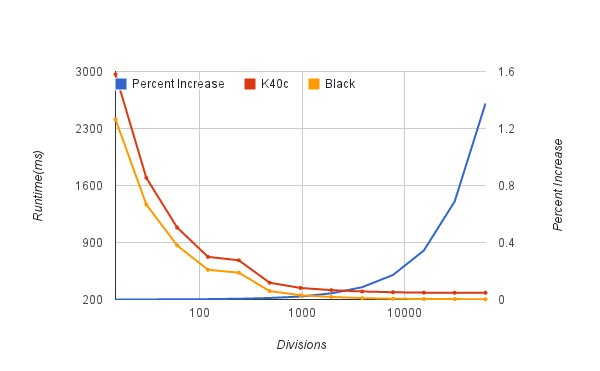
\includegraphics[width=1.0\textwidth]{images/lzchart.png}
\caption{The effects of chunk size on percent increase and runtimes}
\label{fig:lzchart}
\end{figure}

% Please add the following required packages to your document preamble:
% \usepackage{booktabs}
\begin{sidewaystable}[h]
\begin{tabular}{@{}|l|l|l|l|l|l|l|l|l|l|l|l|l|@{}}
\toprule
filename         & \begin{tabular}[c]{@{}l@{}}filesize\\ (MB)\end{tabular} & Black & K40c & lz-og & lz-ansv & plz3 & \begin{tabular}[c]{@{}l@{}}lz-og\\ Speedup\\ Black\end{tabular} & \begin{tabular}[c]{@{}l@{}}lz-ansv\\ Speedup\\ Black\end{tabular} & \begin{tabular}[c]{@{}l@{}}plz3\\ Speedup\\ Black\end{tabular} & LZ      & PLZ     & \begin{tabular}[c]{@{}l@{}}percent\\ increase\end{tabular} \\ \midrule
10Mrandom    & 9.5                                                     & 0.3   & 0.4  & 4.7   & 4.0     & 0.4  & 15.85                                                           & 13.47                                                             & 1.48                                                           & 1426311 & 1426496 & 0.013                                                      \\
chr22.dna    & 33.0                                                    & 1.1   & 1.4  & 22.0  & 19.4    & 1.6  & 20.73                                                           & 18.28                                                             & 1.48                                                           & 2461478 & 2461728 & 0.010                                                      \\
howto.txt    & 37.6                                                    & 1.3   & 1.6  & 25.5  & 24.0    & 1.8  & 20.03                                                           & 18.85                                                             & 1.43                                                           & 3063929 & 3064227 & 0.010                                                      \\
jdk13c       & 66.5                                                    & 2.3   & 2.9  & 41.4  & 40.4    & 2.9  & 18.10                                                           & 17.66                                                             & 1.25                                                           & 1209676 & 1210015 & 0.028                                                      \\
wikisamp.xml & 95.4                                                    & 3.4   & 4.3  & 61.4  & 59.9    & 4.0  & 18.21                                                           & 17.76                                                             & 1.20                                                           & 2888810 & 2889040 & 0.008                                                      \\
w3c2         & 99.4                                                    & 3.9   & 5.0  & 84.1  & 63.1    & 4.4  & 21.55                                                           & 16.17                                                             & 1.13                                                           & 2340638 & 2341016 & 0.016                                                      \\
etext99      & 100.4                                                   & 4.0   & 5.2  & 75.2  & 69.9    & 4.8  & 18.97                                                           & 17.63                                                             & 1.21                                                           & 8306413 & 8306658 & 0.003                                                      \\
sprot34.dat  & 104.5                                                   & 4.1   & 5.2  & 72.2  & 69.0    & 4.6  & 17.69                                                           & 16.90                                                             & 1.13                                                           & 6395921 & 6396224 & 0.005                                                      \\
rctail96     & 109.4                                                   & 4.1   & 5.2  & 96.5  & 70.0    & 4.8  & 23.54                                                           & 17.07                                                             & 1.16                                                           & 3905843 & 3906149 & 0.008                                                      \\
rfc          & 111.0                                                   & 4.3   & 5.5  & 76.6  & 72.8    & 4.8  & 17.81                                                           & 16.93                                                             & 1.12                                                           & 5656068 & 5656367 & 0.005                                                      \\ \bottomrule
\end{tabular}
\caption{Sizes, running times(seconds), and speedups of datasets for evaluation of LZ factorization. GPU implementations use PLZ with 480 divisions}
\label{tab:lzdata}
\end{sidewaystable}

To directly compare the generation of PLZ to algorithms and implementations generating the ideal LZ factorization would be unfair.
The outputs are totally different, as the PLZ has lost an important property of the ideal LZ factorization, the LPF.
The LPF in the PLZ are no longer the longest, as discussed in our implementation.
What can be done is a relative comparison to previous implementations.
We will present the percent increase of the PLZ from the LZ factorization to help in the evaluation.

The data set and CPU benchmarks will be taken directly from the results in \cite{ }. 
Specifically, we will compare our results to their benchmarks of LZ-OG, the most time efficient algorithm as seen in \cite{ }, LZ-ANSV, the sequential algorithm which computes the LZ factorization without every LPF value using lazy LZ factorization, and their contribution PLZ3, their parallel CPU algorithm using 40 cores with hyper-threading.
LZ-ANSV is the closest sequential algorithm after the ANSV generation, while the ANSV generation algorithm comes from PLZ3.

The first and most important metric to look at is how the PLZ chunk size affects the final LZ factorization size.
If the percent increase is too great, then the usage of PLZ is unacceptable.
What percent increas is too great is a judgement that must be made by each user, as each user will have their own requirements.
To pick the different chunk sizes, we decided to use number of divisions as the parameter, although we could have used the actual block size as mentioned before.
More specifically we used multiples of the number of SMs (15).
To try and get a wide range, we used powers of 2 to multiply.

The second most important metric is how the chunk sizes affect the runtimes. 
Since the suffix array construction and the ANSV generation are unrelated, we will keep our focus on the LPF time.
This time assumes the suffix array and ANSV arrays are already present on GPU memory.
It includes the generation of the necessary LPF and PrevOcc arrays, the isolation of the needed values using CUB's deviceSelect, and the data copy of those values back to the CPU.
Many LZ factorization papers evaluate the runtime of their algorithm starting after the suffix array is in memory.
We will consider that runtime later.

Figure~\ref{fig:lzchart} presents the results with these two metrics together.
We show the effect of percent increase and runtime as a function of the number of divisions.
First, we notice that the percent increase grows linearly with the number of divisions.
This trend is intuitive as each extra division has a chance to increase the final PLZ length if the division boundary occurs between the ideal LZ factorization.
Next, we notice that the runtimes generally decreases rapidly as we increase the number of divisions.
At some point however, the rapid decreases stops and increasing the divisions further does not have as much effect on the runtime.
As we can see in Figure~\ref{fig:lzchart}, this occurs at around 480 divisions for both cards.
At 480 divisions the datasets have 0.01 average percent increase.
For some perspective, a file that compresses to 1 MB using the ideal LZ factorization would require an additional 105 bytes using PLZ.
At this point, the Black has an average runtime of 303.7 ms, while the K40c has an average runtime of 406.8 ms.
As we increase the number of divisions from 480 to 30720, Black's runtime decreases only 30 percent, while the percent increase changes over 150 percent to 1.54 percent.
Similarly, K40c's runtime decreases only 32 percent.
We will use this 0.01 percent increase with 480 divisions for the rest of this evaluation.

We now take a look at how our GPU implementation compares to the CPU LZ factorization implementations mentioned earlier.
Table~\ref{tab:lzdata} tabulates the results and speedups found in our experiments.
Our GPU implementation outperforms LZ-OG and LZ-ANSV on all the data sets.
Black sees speedups between 15-24x compared to LZ-OG and speedups between 13-19x compared to LZ-ANSV.
When compared to the 40 core PLZ3 implementation, Black performs comparatively with speedups of 0.1-0.5x.
The slower, K40c sees speedups of 12-19x and 10-15x against LZ-OG and LZ-ANSV respectively.
K40c performed comparatively with PLZ3 having speedups and slowdowns no more than 0.2x.

\begin{figure}[ht!]
\centering
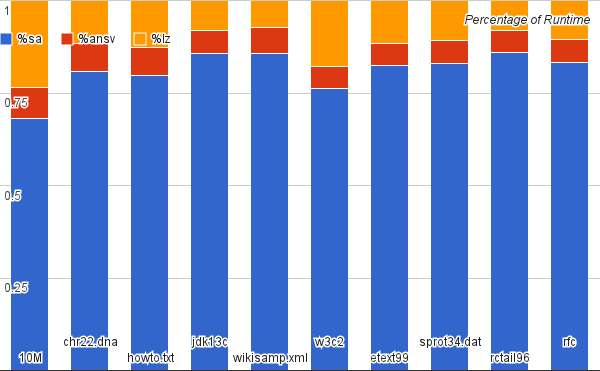
\includegraphics[width=1.0\textwidth]{images/allprof.png}
\caption{Profile of GPU implementation}
\label{fig:allprof}
\end{figure}

Figure~\ref{fig:allprof} shows a profile of the three main sections of our implementation, the SA, the ANSV, and the LZ.
The majority of our implementation, like most LZ factorization implementations, spend most of their time constructing the suffix array.
The suffix array construction takes on average 81 percent of the overall time.

Highly compressible inputs are excluded from the results.
These files incur an incredible space cost when using PLZ, as each division is likely to add an additional factor to the factorization.
An additional factor with a highly compressible input could and probably will result in very high percent increases.

\chapter{Conclusion}
\label{chap:conclusion}

We have presented an algorithm and implementation to calculate the Lempel-Ziv factorization on the GPU.
We show the usage of PLZ in the calculation of the LZ factorization.
Although this removed our ability to calculate the ideal LZ factorization that would be calculated in a traditional sequential algorithm, we found that using the PLZ found significant speedups on the GPU, while incurring a minimal space cost.
Specifically in our evaluation, we found using 480 divisions only increased the LZ factorization by 0.01 percent.
Using 480 divisions, we were able find speedups on an NVIDIA GTX TITAN Black of 15-24x over the sequential LZ-OG algorithm and up to 0.5x over the multicore parallel PLZ3.
Using the PLZ, although not calculating the most space efficient ideal LZ factorization, could work well where time is a more important factor.

We have also presented a reimplementation and reevaluation of the GPU suffix array construction algorithm of Deo and Keely \cite{Deo}.
With the use of GPU libraries and parallel primitives, we were able to replicate their OpenCL results using CUDA on a NVIDIA GPU.
On files greater than 10 MB, we found at least a 4-5x speedup over the fastest CPU implementations.
This suffix array algorithm and implementation have many applications outside of data compression, most notably in bioinformatics.

\chapter{Future Work}
\label{chap:futurework}

Our implementation, like many other LZ factorizaton implementations, was just a proof of concept to show compression speeds and compression ratio.
Although we do output the correct pairs needed, we could take it further and encode them in a way that decompressers can understand.
In doing so, we could create an actual utility to be used to compress actual data.

One aspect that was not considered in this thesis was the effect of having previous knowledge of the input.
Specifically, what can we do if we know the alphabet of the input is limited.
For instance during the suffix array construction, we do an initial sort of the 2/3 group using a 3 character prefix.
To do this, we need to use three radix sorts.
If we know exactly how many bits represent the largest character or integer in the alphabet, we can specialize the radix sort to only sort on those bits.
If this is not possible, we could also check if three characters could fit into a smaller number of characters and perform a lesser number of radix sorts on them.

Recent work has looked at different ways to solve the ANSV problem.
Work done in \cite{Computing longest previous factor in linear time and applications} and \cite{Simpler and Faster Lempel Ziv Factorization} has explored a technique called peak elimination to solve the ANSV problem.
It is unclear whether this solution would parallelize and fit on the GPU architecture.
They also found success using a single data strucute to hold both the PSVs and NSVs to improve memory locality.

Another very important measurement that we did not consider was the space efficiency of our algorithm.
As inputs, such as DNA sequences, grow larger and larger, it is important to make sure the algorithm is as space efficient as possible, so that the algorithm can scale.
Recent work by \cite{Space Efficient Linear Time Lempel-Ziv Factorization on Constant Size Alphabets} has shown methods to reduce the space needed by LZ factorization algorithms by reusing the space required by auxillary data structures.
It is especially important when working on the GPU, where hardware limits are stricter, memory is more sparse, and the communication overhead to go back and forth from the GPU to the CPU is expensive.

Multiple GPU support is becoming increasingly popular as GPU applications become more mainstream.
Enabling multiple GPU support would allow our implementation to handle larger inputs.
It would be interesting to investigate the added communication overhead and its effects on the overall performance.
Multiple GPU support would also allow us to accompany high performance users, who have machines or clusters of machines with single or multiple GPUs.

A simpler optimization that could be added in future implementations is a more dynamic and adaptable kernel launch parameters.
In our implementation, we left many of the kernel paramters as program launch parameters for exhaustive trial and error.
Other kernel parameters were also optimized specifically to the GPU we used for evaluation.
Our implementation would still work with other GPUs, but different parameters might find faster compression speeds.
One approach is to gather information about the GPU using the CUDA API before launching any kernels.
We can then use that information to generate more sensible grid and block sizes.
We can also use templating features for greater flexibility.
Many CUDA libraries make use of this approach to great success.

NVIDIA CUDA is still a growing framework, as new hardware and new API releases add additional features to ease or enable programmers.
Recent releases have enabled dynamic parallelism and a unified memory.
Dynamic parallelism allows GPU kernels to launch additional kernels from the kernels themselves.
Traditionally, the GPU is used as a coprocessor and kernels must be launched from instructions on the CPU.
Using dynamic parallelism, added overhead from communication between the GPU and CPU can me circumvented.
Dynamic parallelism can also allow for easier or more load balanced parallelism.
For example, during the final LZ factorization calculation, we could launch a new CUDA kernel to do string comparisons instead of having threads in a block working together.
The benefits of unified memory in our current implementation is not clear.
Since most of the data is generated and remains on the GPU, unified memory may only simplify the communication while not adding performance benefits.
It would still be interesting to evaluate if these new features could provide speedups.

As of now, our implementation works only on NVIDIA GPUs through the use of CUDA.
Although GPGPU development is dominated by NVIDIA CUDA on NVIDIA GPUS, the graphics market share includes many other significant vendors, including AMD and Intel.
There are a variety of methods to create an implementation for use with those other vendors.
The first is to rewrite the implementation using OpenCL.
OpenACC, GPU Ocelot
Furthermore, the usage of PLZ could be examined on different platforms, where the cost to perform string comparisons are not as expensive, like a multicore CPU.



% ------------- End main chapters ----------------------

\clearpage
\nocite{*}
%\bibliographystyle{plain}
\bibliography{Bibliography}
%\addcontentsline{toc}{chapter}{Bibliography}

%\begin{appendix}
%%\addcontentsline{toc}{chapter}{\appendixnamelower}
%\include{Appendix}
%\end{appendix}

\end{document}
